\newpage
\section{Experiment Definition}
\begin{table*}[ht]
    \centering
    \begin{tabularx}{\textwidth}{@{}p{4.5cm} p{6cm} p{6cm}@{}}
        \hline
        \textbf{Goal} & \textbf{Research Questions} & \textbf{Metrics}\\
        \hline
        \midrule
        Quantify the impact of quantization on server-hosted LLMs (Granite-7B, LLaMA-2 7B, Mistral-7B) with respect to energy, accuracy, efficiency, and carbon emissions. & MRQ: How does quantization affect energy, accuracy, and resource utilization in LLMs? & Energy, Carbon: kWh, J, gCO$_2$ = Ci × E
        Time: latency (ms), throughput (tokens/s)\\
        \hline
         & RQ1: How to build a benchmarking system for baseline vs. quantized LLMs? & Resources: GPU\% / GPU memory (GB) / CPU\%\\
         \hline
         & RQ2: What are the accuracy–efficiency trade-offs? & Accuracy: MMLU (Acc\%)\\
         \hline
         & RQ3: Which model family benefits most from quantization? & Trade-offs: \% differences vs. baseline; accuracy–energy, latency–accuracy curves\\
         \hline
         & RQ4: How do carbon emissions vary under different grid conditions? & favourable (off-peak, renewable), unfavourable (peak, fossil-heavy)\\
         \hline
         \bottomrule
    \end{tabularx}
    \caption{GQM Summary - Server-side Quantization of LLMs}
    \label{tab:placeholder}
\end{table*}

\begin{figure}[t]
    \centering
    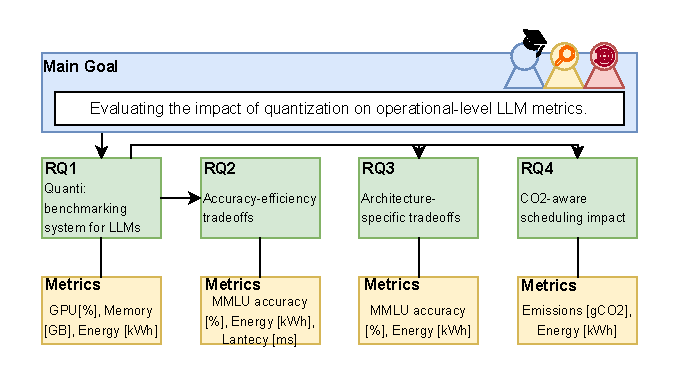
\includegraphics[width=1.05\linewidth]{reportTemplate/figures/gqm.pdf}
    \caption{Goal-Question-Metric (GQM) framework overview this work follows. Stakeholders from multiple groups, especially students, LLM operators, and sustainability drivers could benefit from the software and the data produced in this work and released as open-science.}
    \label{fig:placeholder}
\end{figure}

% Report about the GQM (with figure).
In this section, we define the experiment and multi-layer analyze following the GQM-model for experimentation. Overall, in \Cref{sec:experiment:goal}, we identify the main goal of analyzing the impact of LLM compression by quatization on sustainability and performance metrics. To achieve these, we formulate and answer one main research question, and further divide into three sub-research questions; in \Cref{sec:experiment:questions}, we present the research questions that guide our experiments. Then, in \Cref{sec:experiment:metrics}, we present and expand on the metrics we use to quantify energy consumption, resource utilization, and accuracy.

\subsection{Goal}\label{sec:experiment:goal}
LLMs are widely adopted at the societal scale, and raise performance and efficiency concerns, further cascading into sustainability concerns. Addressing this challenge, LLM researchers, engineers, and operators adopt quantization as a compression technique, which is expected to alleviate the efficiency concerns~\cite{zhang2023dual, DBLP:conf/icml/NagelABLB20}. However, it is still underexplored in the scientific community how quantization impacts performance, efficiency, and sustainability. 

We thus identify the main goal of 
\textit{(MG) evaluating the impact of quantization on operational-level LLM metrics.} Achieving the main goal, and, thus, answering the main research question (MRQ), would benefit stakeholders from various groups; for example, operations could gain deployment insights into compressed LLMs; sustainability operators would gain insights into the importance of CO2-aware workload scheduling against LLM ``optimization"\footnote{This term comes in quotes due to its invalidity, but its widely usage. We argue that 1) since optimization means making something optimum, thus perfect, and 2) since nothing is either optimum or perfect in Computer Science, the term ``optimization" is invalid in our field.} techniques (e.g., compression by quantization; researchers and students can use the open-source benchmarking tool Quanti for exploration in the field.

We further identify the goal 
(G1) of designing and implementing a benchmarking system for quantifying LLMs, which would aid the experimentation process of identifying and evaluating impacts and tradeoffs.

We identify (G2) of evaluating how compression by quantization impacts operational-level metrics of LLMs, and hence comprehend how quantization can impact the real-world operation of these systems. 

Furthermore, we identify the goal 
(G3) of quantifying how accuracy impacts the energy consumption of LLMs, especially when LLMs differ in architecture (e.g., LLama2:7B from Meta underlies a different architecture than Granite:7B from IBM). While it is expected that higher accuracy requires higher computational power, and thus more energy consumption, it is yet unclear whether there is a relation, and to what extent, between accuracy and energy consumption. 

CO2-aware scheduling is widely employed in datacenter operation to meet Service Level Objectives and reduce the environmental footprint of massive-scale systems~\cite{DBLP:journals/corr/abs-2206-03259, nicolae5377101m3sa, DBLP:conf/wosp/NiewenhuisTIM24}. Following a similar approach, we identify the goal of evaluating CO2-aware scheduling of LLM inference; we thus explore, through (G4), the impact of running an LLM compressed by quantisation, which is expected to consume fewer resources, yet at an unfavourable CO2-intensity timestamp, against running inference through an uncompressed LLM, which is expected to consume more resources, yet at a favourable CO2-intensity timestamp. Through this goal, we aim to analyze the importance of CO2-aware scheduling against compression techniques.


\subsection{Questions}\label{sec:experiment:questions}

We identify the main research question: \textit{\textbf{(MRQ)} How to explore the impact of compression by quantization of LLMs and how this technique impacts energy consumption, resource utilization, and precision?}

To answer MRQ, we identify four decomposed research question, each corresponding to the goals identified in \ref{sec:experiment:goal}:

\textit{\textbf{(RQ1)} How to design and implement a benchmarking system for quantifying LLMs?} The essence of RQ1 involves designing and establishing the benchmarking tools for explainable and reproducible experimentation. To answer RQ1, also linked to G1, we propose Quanti, a benchmarking tool which aids in assessing, quantifying, and comparing the effects of LLMs quantization (\Cref{sec:design}).

\textit{\textbf{(RQ2)} How to evaluate the impact of compression by quantization on operational-level metrics of LLMs}. The essence of RQ2 involves examining the direct effects of quantization on sustainability and performance indicators of LLMs and quantify the magnitude of change when tranisioning from basedline to quantized model configurations. To answer RQ2, also linked to G2, we employ an engineered prototype of Quanti and measure energy consumption and inference time of four LLMs of identical size (i.e., same number of parameters), with and without quantization applied (\Cref{sec:experiments:operational-level}).

\textit{\textbf{(RQ3)} How to evaluate the tradeoff accuracy-energy consumption across various-architecture LLMs with and without compression by quantization?} The essence of RQ3 involves examining the effects of quantization on performance-level and sustainability-level indicators and identifying correlations. To answer RQ3, also linked to G3, we select four LLMs, of different architectures, and identify whether (and to what extent) arhitectural differences (e.g., LLaMA-2, Granite, Mistral) influence the trade-off characteristics (\Cref{sec:experiments:accuracy-energy}.

\textit{\textbf{(RQ4)} How to evaluate the impact of carbon intensity for compressed and uncompressed models at favourable and unfavourable carbon intensity day instances?} The essence of RQ4 is analysing (aimed at proving) the importance of workload scheduling CO2-awarely. To answer RQ4, also linked with G1, we select one LLM, a monthly CO2 intensity trace, and measure energy consumption. We compare the relative difference in CO2 emissions for running the same workload task on a baseline LLM at the CO2-best-overall CO2 intensity time interval of the day and on a quantised LLM at the CO2-worst-overall time interval(\Cref{sec:experiments:co2-aware}.

% \begin{itemize}
% \item \textbf{MRQ:} How to explore the impact of compression by quantization of LLMs and how this technique impacts energy consumption, resource utilization, and precision

% \item \textbf{RQ1:} How to design and implement a benchmarking system for quantifying LLMs?
% \item \textbf{RQ2:} How to evaluate the impact of compression by quantization of operational-level metrics of LLMs?

% \item \textbf{RQ3:} How to evaluate the tradeoff accuracy-energy consumption across various-architecture LLMs under quantization and without quantization?

% \item \textbf{RQ4:} How to evaluate the impact of carbon intensity for compressed and uncompressed models at favourable and unfavourable carbon intensity day instances?


% \end{itemize}

%  - Our main question comprises of how we assess the impact of quantization on LLMs (e.g LLama2 7B, Granite 7B, and Mistral 7B) and how it effects the energy usage (kWh, Joules), inference time (ms), accuracy (percent) and resource utilization (CPU/GPU load percent or memory in GB) when deployed on server based system. 

% sub questions:

% - to design a benchmarking system that supports systematic evaluation of energy usage (kWh), inference latency (ms), resource utilization (CPU/GPU percent and memory GB) and accuracy trade-offs

% - How can we identify and quantify the trade-offs between accuracy and efficiency when comparing baseline and quantized models specifically in terms of reduced energy use (kWh, Joules) and memory footprint (GB) versus possible accuracy drops in percent.
%  for example, quantization can reduce energy usage and may be memory, but it can drop the accuracy. so the objective of this question is to understand the sweet spot between sustainability and performace.

% - 


% - to identity which llm model shows benefits (in terms of sustainability and perfomance) from quantization. so the idea is to see wether Granite, LLaMA or Mistral will get the energy savings, effiency with accuracy, as not all models will be same to get these benefits.

% - Similarly, to evaluate the carbon intesity of baseline and quantized models at different time periods of the day (favourable and unfavourable carbon intensity day instances). for example, running the same model at peak grid load vs off-peak renewable heavy hours, may produce differnt carbon footprints. so we can see how quantization interacts with real world energy sourcing .

\subsection{Metrics}\label{sec:experiment:metrics}
To answer the research questions, the experiment will record both operation-level and task-level quality metrics so each is measured with explicit units of measurement for reproducibility.

We will measure energy usage in kilowatt-hours (kWh) and Joules through utilities such as pyJoules, CodeCarbon, or Experiment Runner. This allows us to log the total energy required to execute inference tasks and to scale energy per request or per token.

Inference latency will be tracked along two dimensions: per-prompt latency (milliseconds), measuring responsiveness, and throughput in tokens per second, measuring scalability.

Resource utilization will include GPU utilization (percent), GPU memory utilization (GB), and CPU usage (percent) during inference. These will reflect the performance relative to efficiency in utilization of computational resources when models are quantized versus their baseline equivalents.

Accuracy will be measured with a number of benchmarks, each having domain-agnostic metrics:

- MMLU: Knowledge and reasoning task accuracy (\%).

- TriviaQA: F1 score (percent) and Exact Match (EM) on question answering.

- CNN/DailyMail or XSum: ROUGE and BLEU on summarization.

The intensity of carbon will be measured by transposing energy consumption into equivalent CO$_2$ emissions, per the formula Ce = Ci × E, where Ce is the total emissions (grams CO$_2$), Ci is grid carbon intensity (gCO$_2$/kWh), and E is energy consumed (kWh). For the sake of realism, this will be estimated for optimal (renewable-abundant, off-peak) and extreme (fossil-fuel abundant, peak) grid conditions.

Finally, relative trade-offs among similar levels of performance will be compared by relative percentage differences between baseline and quantized counterparts across all metrics. Accuracy–energy trade-off and latency–accuracy curves will be plotted as well to illustrate sustainability vs. performance trade-offs.





